Ranije su izvedene jednačine(Eulerove) koje opisuju kretanje projektila. U ovim jednačinama se 
pojavljuju sile i momenti koji djeluju na projektil, te je neophodno i njih odrediti kako bi 
se postigao potpun dinamički model projektila. Također, poznavanje prirode ovih sila je neophodno kako 
bi se moglo upravljati projektilom jer se upravo kontrolom ovih sila postiže upravljanje projektila.
Sile koje djeluju na projektil u letu su aerodinamičke, pogonske sile i 
gravitaciona sila. Ove sile se mogu razložiti po osama kooridnatnog sistema vezanog 
za tijelo i mogu se izraziti u inercijalnom kooridnatnom sistemu. 
\section{Gravitaciona sila}
Prije svega važno je istaći da se gravitaciona sila ne može koristiti za upravljanje projektilom i 
ona predstavlja ništa više od vanjske smetnje na sistem automatskog upravljanja.
Gravitaciona sila predstavlja vektor koji je usmjeren ka centru Zemlje i u inercijalnom kooridnatnom
sistemu je dat sa:
\begin{equation}
    G_{z}=[0\;  0\;  mg]^T
\end{equation}
Da bi se dobila vrijednost gravitacione sile u kooridnatnom sistemu tijela, treba se koristiti matrica 
transformacije:
\begin{equation}
    G_{b} = T_{z}^bG_{z}
\end{equation}
Korištenjem \ref{eq:ztob}, dobija se:
\begin{equation}
    G_b = mg\begin{bmatrix}
        -\sin\theta \\
        sin\phi\cos\theta \\
        \cos\phi\sin\theta
    \end{bmatrix}
\end{equation}
Na sličan način, korištenjem \ref{eq:ztov}.  se dobija i vektor gravitacione sile u brzinskom koordinatnom sistemu:
\begin{equation}
    G_v = T_{z}^v\begin{bmatrix}
        0 \\ 0 \\ mg\end{bmatrix} = mg\begin{bmatrix}
            -\sin\Theta \\ 0 \\ \cos\Theta
    \end{bmatrix}
\end{equation}
Gravitaciona sila se u opštem slučaju mijenja u vremenu pošto se masa projektila mijenja usljed utroška goriva
pri letu projektila. Varijacije u gravitacionom ubrzanju se zanemaruju pri promjeni geografske širine.  
Promjena mase projektila je od krucijalne važnosti za balističke projektile kod kojih $90\%$ mase čini gorivo.
\section{Pogonska sila}
Pogonska sila je sila koju generiše mlazni motor projektila. Karakteristike motora zavise 
od zahtjeva vođenja i od prirode mete. Motor se nalazi na stražnjem dijelu projektila i stvara reaktivnu 
silu. Intenzitet ove sile varira u zavisnosti od tipa motora i zadatka projektila. Tipovi projektila mogu biti:
\begin{itemize}
    \item All-boost- ima za posljedicu veliko ubrzanje projektila i kratko vrijeme leta pošto se gorivo potroši u kratkom roku
    \item All-sustain- ima za posljedicu stalnu brzinu projektila i dugo vrijeme leta
    \item Boost-sustain- Ovaj tip motora kombinuje najbolje osobine prethodna dva tipa
\end{itemize}
Ovdje će se pretpostaviti da mlazni motor generiše silu konstantnog intenziteta. Za većinu 
projektila smjer sile se ne mijenja i zbog građe projektila uvijek dujeluje u pozitivnom smjeru 
$X_b$ ose pa je pogonska sila u koordinatnom sistemu tijela data sa:
\begin{equation}
    P_{tijelo}=[P\;  0\;  0]^T
\end{equation}
Pogonska sila izražena u sistemu brzine je data sa:
\begin{equation}
    P_v = T_{b\to v}\begin{bmatrix}
        P \\ 0 \\ 0
    \end{bmatrix} = {T_{v}^b}^T\begin{bmatrix}
        P \\ 0 \\ 0
    \end{bmatrix}
\end{equation}
Pa se dobija:
\begin{equation}
    P_v=P\begin{bmatrix}
        \cos\alpha\cos\beta \\ \cos\alpha\sin\beta \\ -\sin\alpha
    \end{bmatrix}
\end{equation}
\section{Aerodinamičke sile}
Aerodinamička sila je posljedica djelovanja pritiska okolnog fluida na tijelo u pokretu. 
Aerodinamička sila se može razložiti na tri komponente koje su definisane u nastavku:
\begin{itemize}
    \item \textbf{Uzgon}- Uzgon je komponenta rezultantne aerodinamičke sile 
    koja je normalna na relativno kretanje vjetra.
    \item \textbf{Otpor}- Otpor je komponenta rezultantne aerodinamičke sile 
    koja je paralelna relativnom kretanju vjetra.
    \item \textbf{Bočna sila}- Bočna sila je komponenta rezultantne aerodinamičke sile 
    koja je normalna na uzgon i otpor. 
\end{itemize}
Ovdje se posmatraju projektili koji se zakreću da bi skrenuli(skid to turn) i 
kod takvih projektila aerodinamičke sile su date sa:
\begin{equation}
   \text{Otpor} \quad R_x=C_xqS
   \label{eq:aa1}
\end{equation}
\begin{equation}
    \text{Uzgon} \quad R_z=C_zqS
    \label{eq:aa2}
\end{equation}
\begin{equation}
    \text{Bočna sila} \quad R_y=C_yqS
    \label{eq:aa3}
\end{equation}
,gdje su $C_x,C_y$ i $C_z$ aerodinamički koeficijenti, $q$ dinamički pritisak slobodnog strujanaja
u tački daleko od objekta i iznosi $q=\frac{1}{2}\rho v^2$, $S$ je referentna površina i 
$v$ je brzina vazduha, $\rho$ predstavlja atmosferski pritisak.\\
Treba napomenuti da se aerodinamičke sile i momenti izražavaju bezdimenzionalnim veličinama. 
To se postiže tako što se dogovorom utvrdi da se sila(ili moment) predstavlja svojim odgovarajućim 
aerodinamičkim koeficijentom. Prema tome, $C_x$ potpuno određuje silu otpora i slično vrijedi i 
za ostale koeficijente. \\
U opštem slučaju koeficijenti aerodinamičkih sila su funkcije varijabli stanja pa se može
napisati:
\begin{equation}
    C_x=C_x(\alpha ,\beta, M,q,\delta_v,\delta_P,\delta_e)
\end{equation}
,gdje je $M$ Mahov broj- odnos tekuće brzine i brzine zvuka, $\alpha$ napadni ugao i 
$\beta$ ugao klizanja. Slično tako vrijedi:
\begin{eqnarray}
    C_y=C_y(M,\beta,\delta_P)\\
    C_z=C_z(M,\beta,\delta_v)
\end{eqnarray}
Uglovi $\alpha, \beta$ i $\gamma$ su prikazani na slici \ref{fig:angles} i definisani su sa:
\begin{equation}
    \alpha=arctg(w/u)
\end{equation}
\begin{equation}
    \beta=\arcsin(v/v_m)
\end{equation}
\begin{figure}[ht!]
    \centering
    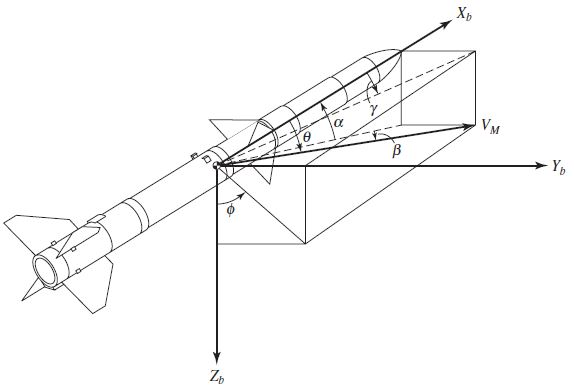
\includegraphics[scale=0.7]{angles.JPG}
    \caption{Ugaone veze}
    \label{fig:angles}
\end{figure}
Dodatno, napadni ugao $\alpha$ definiše rotaciju sistema tijela oko $Y_b$ ose, a ugao klizanja 
$\beta$ definiše rotaciju sistema tijela oko $Z_b$ ose. 
Sada je potrebno poznavati analitičke oblike aerodinamičkih koeficijenata u zavisnosti 
od odgovarajućih varijabli stanja. Linearizacijom aerodinamičkih koeficijanata u okolini trenutnih vrijednosti 
varijabli stanja dobijaju se linearne relacije za aerodinamičke koeficijente koje su 
izražene u obliku sume \textit{aerodinamičkih izvoda} i varijabli stanja.
Razvojem u Taylorov red i odbacivanjem viših članova dobija se aproksimacija 
aerodinamičkih koeficijenata:
\begin{eqnarray}
    &C_x&=C_{x_0}+C_{x_{\alpha\delta _v}}\alpha+C_{x_\alpha^2}\alpha^2-C_{x_{\delta _V^2}}\\
   &C_z&=C_z^{\alpha}{\alpha} + C_z^{\dot{\alpha}} \dot{\alpha}+C_z^q q+C_z^{\delta _v}{\delta _v}\\
    &C_y&=C_y^{\beta}{\beta} + C_y^{\dot{\beta}} \dot{\beta}+C_y^q q+C_y^{\delta _P}{\delta _P}
\end{eqnarray}
,gdje je $C_{x_0}=\frac{\partial c_x}{\partial \alpha}|_{\alpha=0}$, $C_{x_1}=\frac{\partial c_x}{\partial \alpha}$ 
i slično tako za ostale izvode.\\
Također je važno istaći da su ovi koeficijenti(tj. sile) izražene u \textit{kooridnatnom sistemu vjetra} 
relativnom toku vazduha. Često se u literaturi ovi koeficijenti definišu u \textit{kooridnatnom sistemu brzine tijela}, kod kojeg se $X$ osa podudara sa 
brzinom letjelice, ali zbog pretpostavke da je brzina vjetra zanemariva u inercijalnom kooridnatnom sistemu razlika 
u ovim koordinatnim sistemima ne igra ulogu. 
Izuzetno je korisno imati i vrijednosti aerodinamičkih sila u koordinatnom sistemu 
tijela. One su date sa:
\begin{align}
    \begin{bmatrix}
        F_{ax}\\F_{ay}\\F_{az} 
        \end{bmatrix}
        &= -\frac{\rho v_m^2\pi D^2}{8}\begin{bmatrix}
        C_{x0} + \alpha^2+\beta^2\\C_{NA}\alpha\\C_{NA}\beta
        \end{bmatrix}
\end{align}
%Sada se vraćanjem u \ref{eq:aa1},\ref{eq:aa2} i \ref{eq:aa3} mogu odrediti 
%aerodinamičke sile koje djeluju na projektil. 
\section{Aerodinamički momenti}
Momenti se mogu podjeliti na momente koji su posljedica aerodinamičkog tereta i 
pogonske sile koja ne djeulje kroz centar gravitacije. Moment koji je posljedica 
rezultantne sile koja ne djeluje na centar kooridnatnog sistema tijela se može 
podjeliti na tri komponente, i to:
\begin{itemize}
    \item \textbf{Moment valjanja} je moment oko lateralne ose($Y_b$) projektila i generisan 
    je od uzgonom i otporom koje djeluju na tijelo. Pozitivan moment je u smjeru gore 
    od nosa letjelice 
    
    \item \textbf{Moment propinjanja} je moment oko longitudinalne ose($X_b$) projektila.
    Posljedica je uzogna koji je uzrokovan nekom vrstom elerona. Pozitivan moment propinjanja uzrokuje kretanje nadole 
    desnog krila.
    
    \item \textbf{Moment zakretanja} je moment oko vetikalne ose projektila($Z_b$). Pozitivan moment zakretanja 
    ima za posljedicu da se nos aviona zakrene u desno. 
\end{itemize}
Kvantitativno, momenti su dati sa:
\begin{equation}
    \text{Moment valjanja} \quad L=C_lqSb
    \label{eq:a1}
 \end{equation}
 \begin{equation}
     \text{Moment propinjanja} \quad M=C_mqSc
     \label{eq:a2}
 \end{equation}
 \begin{equation}
     \text{Moment zakretanja} \quad N=C_nqSb
     \label{eq:a3}
 \end{equation}
 ,gdje je $b$ raspon krila, $c$ je razmak između početne i krajnje ivice krila mjerene 
 u smjeru paralelnom toku vazduha, $S$ je površina platforme krila. 
 Isto kao i kod slučaja sa silama, koeficijenti momenata također zavise od više promjenjivljih 
 i potrebno ih je linearizirati. \\
 Linearizirani koeficijenti momenta  su:
 \begin{equation}
     C_M=C_M^{\alpha}\alpha +C_M^{\dot{\alpha}}\dot{\alpha} + C_M^Q Q/(2v_m)+C_M^{\delta _v}\delta _v
 \end{equation}
 ,koeficijent momenta skretanja je:
 \begin{equation}
     C_N=C_N^{\beta}\beta + C_N^{\dot{\beta}}\dot{\beta}+C_N^R R/(2v_m)+C_N^{\delta _P}\delta _P
 \end{equation} 
 Pri čemu je za krstastu konfiguraciju $C_M^{\alpha}=C_N^{\beta}$, $C_N^{\dot{\beta}}=C_M^{\dot{\alpha}}$,
 $ C_M^Q=C_N^R $, $C_M^{\delta _v}=C_N^{\delta _P}$.
 Koeficijent momenta valjanja se linearizuje tako da se dobije:
 \begin{equation}
     C_L = C_L^PP/(2v_m)+C_L^QQ/(2v_m)+C_L^RR/(2v_m) +C_L^\alpha \alpha +C_L^\beta \beta + C_L^{\delta _e} \delta _e +C_L^{\delta _v} \delta _v
     +C_L^{\delta _P} \delta _P
 \end{equation}
 Važno je istaći da se kod proračuna momenta valjanja ističu samo koeficijenti $C_L^P$ i $C_L^{\delta _E}$ a u nekim analizama 
 se uzimaju i koeficijenti $C_L^\alpha$ i $C_L^\beta$. Prema tome, koeficjent momenta 
 valjanja se približno može izraziti kao:
 \begin{equation}
    C_L \approx C_L^PP/(2v_m)+C_L^{\delta _e} \delta _e
 \end{equation}
 Najvažnije od svega je činjenica da su aerodinamički momenti posljedica 
 geometrijskog razmaka centra gravitacije i napadne tačke aerodinamičkih sila(tj. centra pritiska).
 Ova razlika se izražava preko veličine zvane \textit{statički stabilitet}. Konkretno, vrijedi:
\begin{align}
    C_M^\alpha &= C_z^\alpha(X_{cg}-X_{cp})/C\\
    C_N^\beta &= C_y^\beta(X_{cg}-X_{cp})/C
\end{align}
Fizikalna interpretacija statičkog stabiliteta je takva da ako letjelica ima centar gravitacije bliže nosu nego 
centar pritiska, da će letjelica sama po sebi doći u stcionarno stanje nakon svakog prelaznog procesa. 
Konkretno, komercijalni avioni imaju relativno veliki statički stabilitet. Oni se odlikuju sporim i stabilnim 
prelaznim procesima. S druge strane, borbeni avioni(npr. F22 Raptor) imaju relativno mali statički stabilitet ili su 
nestabilni. Ovo je posljedica potrebe za agresvnim manevrima u toku borbe. Pošto se ovakve letjelice odlikuju brzim prelaznim 
procesima, neophodno je u svakom trenutku korigovati otklon kontrolnih površina što pilot ne može samostalno uraditi. 
